\Lecturer{Hui Jin}
\Contributor{}
\LectureNumber{14}
\LectureDate{DATE}
\LectureTitle{Quantum Error Correction Codes}

\lstset{style=mystyle}


	\MakeScribeTop

%#############################################################
%#############################################################
%#############################################################
%#############################################################

\section{Introduction}
Despite the great promise held by the quantum computing, quantum noise poses a major challenge in the development of quantum computers as it can cause qubits to lose their delicate quantum state, known as decoherence.

Quantum Noise refers to the unwanted disturbances that affect quantum systems, leading to errors in quantum computations. Unlike classical noise, which might simply add random errors to a signal, quantum noise can have more complex and detrimental effects. 

Quantum noise can arise from various sources, including thermal fluctuations, electromagnetic interference, imperfections in quantum gates, and interactions with the environment. Different types of quantum noise affect qubits in distinct ways. For example, phase noise alters the relative phase between the basis states of a qubit, while amplitude noise affects the probabilities of measuring different states. 

Quantum noise creates a significant barrier to the development of large-scale, fault-tolerant quantum computers. Even small amounts of noise can lead to decoherence, causing qubits to lose their superposition and entanglement properties. This loss of quantum information can render computations meaningless and limit the size and complexity of feasible quantum algorithms. 


Efforts to mitigate quantum noise include improving the physical isolation of qubits, developing more precise control techniques. The most promising technique among them is quantum error correction codes, which is our focus here. 


Quantum error correction (QEC) is used in quantum computing to protect quantum information from errors due to decoherence and other quantum noise. Quantum error correction is essential to achieve fault tolerant quantum computing that can reduce the effects of noise on stored quantum information, faulty quantum gates, faulty quantum preparation, and faulty measurements. This would allow algorithms of greater circuit depth and allow us build large scale quantum computers.

Error correction itself is not a new concept; classical error correction codes started around the year of 1948, when Shannon invented the channel coding theory and Hamming independently created the first non-trivial code Hamming code. Quantum error correction (QEC) requires much more thought. On a fundamental level, standard classical error correction only needs to correct bit flip errors, where bits accidentally switch from \(0\) to \(1\) or vice versa. Such error are digitized and big. Quantum computers must correct more kinds of errors, like phase errors which can corrupt the extra quantum information that qubits carry and does not have a counterpart in the classical world. Not only that, but QEC techniques must correct errors without the ability to copy unknown quantum states, and without destroying the underlying quantum state.

In particular, the no-cloning theorem was a huge barrier to introduce the techniques in classical error correcting codes into the quantum world. The essence of classical error correction codes rests on the notion of duplication, or repetition. From the simplest repetition codes, to the state-of-the art low-density parity-check nodes, irregular repeat accumulate codes, repetition is an indispensable component of the code construction for structured redundancy. Since the no-cloning theorem say duplicating the qubit \(\ket{\phi}\) is not possible, how can we add redundancy? Miraculously, the quantum entanglement provides a solution.
 
 Another thorny obstacle in quantum error correcting codes is related to measurement.   If an error does occur on our encoded state, the natural thing to do is to perform a measurement on the state in order to diagnose the error. For example, the majority vote decoding algorithm for the repetition code relies on this simple concept. However, in the quantum world, measurements collapses the state and destroys the information we were trying to protect. To handle this problem, we use syndrome decoding where only error patterns are measured. Without measuring the data we do not collapse the quantum states. 

Let’s summarize the essential ideas that underlie the quantum error correction scheme:
\begin{itemize}
    \item The errors are digitized. Although the errors in the quantum information
were small, we performed measurements that projected our state onto either a state with no error, or a state with one of a discrete set of errors that we knew how to convert.

\item The errors are measured without measuring the data. Our measurements revealed the nature of the errors without revealing (and hence disturbing) the encoded information.

\item The errors are local, and the encoded information is nonlocal. It is important to emphasize the central assumption underlying the construction of the code – that errors affecting different qubits are, to a good approximation, uncorrelated. We have tacitly assumed that an event that causes errors in two qubits is much less likely than an event causing an error in a single qubit. It is of course a physics question whether this assumption is justified or not – we can easily envision processes that will cause errors in two qubits at once. If such correlated errors are common, coding will fail to improve reliability.
\end{itemize}

\section{No Cloning Theorem}
No cloning theorem says nature prevents us duplicating a general qubit.  
\begin{theorem}
In general we cannot clone a qubit unless it is a pure state.    
\end{theorem}

\begin{proof}
Let us assume that there exists an operation \(U_{cl}\) that we can apply to clone any qubit \(\ket{\phi} = \alpha \ket{0} + \beta \ket{1}\) to a pure state \(\ket{0}\), for arbitrary complex numbers \(\alpha, \beta\). That means we have 
\[U_{cl}(\ket{\phi}\ket{0}) = \ket{\phi}\ket{\phi},\]
for any qubit \(\ket{\phi}\).

If we expand the qubit \(\phi\) after the cloning, we have 
\begin{align*}
    U_{cl}(\ket{\phi} \ket{0}) &= \ket{\phi}\ket{\phi} \\
           &= (\alpha \ket{0} + \beta \ket{1})(\alpha \ket{0} + \beta \ket{1}) \\
           &= \alpha^2 \ket{00} + \alpha\beta\ket{01} + \alpha\beta\ket{10} + \beta^2 \ket{11}
\end{align*}

However, if we expand qubit \(\ket{\phi}\) first, and apply the cloning on the pure state, due to the linearity of quantum operation, we have 
\begin{align*}
   U_{cl} (\ket{\phi} \ket{0})  &= U_{cl}((\alpha \ket{0} + \beta \ket{1}) \ket{0}) \\
           &= \alpha U_{cl}(\ket{0}\ket{0}) +  \beta U_{cl}(\ket{1}\ket{0}) \\
           &= \alpha \ket{00} + \beta \ket{11}
\end{align*}
which does not have the cross states \(\ket{01}\) \(\ket{10}\). This is a contradiction unless \(\alpha\) or \(\beta\) equals to zero. 
\end{proof}

Since duplication, or repetition, is such a fundamental idea in error correcting code, the no-cloning theorem seemingly dealt a blow to the idea of quantum error correcting codes.

\section{Channel Noise Models}

\subsection{Bit-flip Noise}
The bit-flip noise converts the qubits 
\(\ket{0}\) and \(\ket{1}\) into each other. Hence, the original qubit \(\ket{q} = \alpha \ket{0} + \beta \ket{1}\) is distorted by the quantum noise into \(\ket{q} = \alpha \ket{1} + \beta \ket{0}\). We can think of the bit flip noise as transforming the original qubit by a Pauli matrix \(\sigma_X\).

This noise is similar to the binary symmetric channel in the classical world. 

Note that for the alternative basis states \(\ket{+}\), the bit-flip noise has no effect; for \(\ket{-}\), the bit=-flip noise changes the sign. 
In summary, we have:
\begin{align*}
    \sigma_X \ket{0} &= \ket{1} \\
    \sigma_X \ket{1} &= \ket{0} \\
    \sigma_X \ket{+} &= \ket{+} \\
    \sigma_X \ket{-} &= -\ket{-}
\end{align*}

\subsection {Phase Flip Noise}
A phase flip noise changes the phase of a qubit. For the base states, we have 
\(\ket{0} \rightarrow \ket{0}\), but \(\ket{1} \rightarrow - \ket{1}\).

Hence, the original qubit \(\ket{q} = \alpha \ket{0} + \beta \ket{1}\) is transformed by the quantum phase noise into \(\ket{q} = \alpha \ket{0} - \beta \ket{1}\); so the channel  introduces a dephasing factor \(e^{i\pi}\) between the two complex amplitudes \(\alpha, \beta\).

Note that for the alternative basis states \(\ket{+}\), the bit-flip noise changes it to \(\ket{-}\); for \(\ket{-}\), the bit-flip noise changes it to \(\ket{+}\). 


We can think of the phase flip noise as transforming the original qubit by a Pauli matrix \(\sigma_Z\).

This noise has no counterpart in classical world. 

In summary, we have:
\begin{align*}
    \sigma_Z \ket{0} &= \ket{0} \\
    \sigma_Z \ket{1} &= -\ket{1} \\
    \sigma_Z \ket{+} &= \ket{-} \\
    \sigma_Z \ket{-} &= \ket{+}
\end{align*}

With a clever trick, we can treat the phase-flip noise as bit-flip noise. In fact, we can verify that 
\begin{align*}
    \sigma_X = H \sigma_Z H \\
\end{align*}
By appending a Hadamard transformation before and after a channel noise \(\sigma_Z\), we have effectively a bit flip noise channel. This is illustrated in Figure~\ref{fig:QEC_BitFlipEquivalence}.

\begin{figure}[ht]
\centering
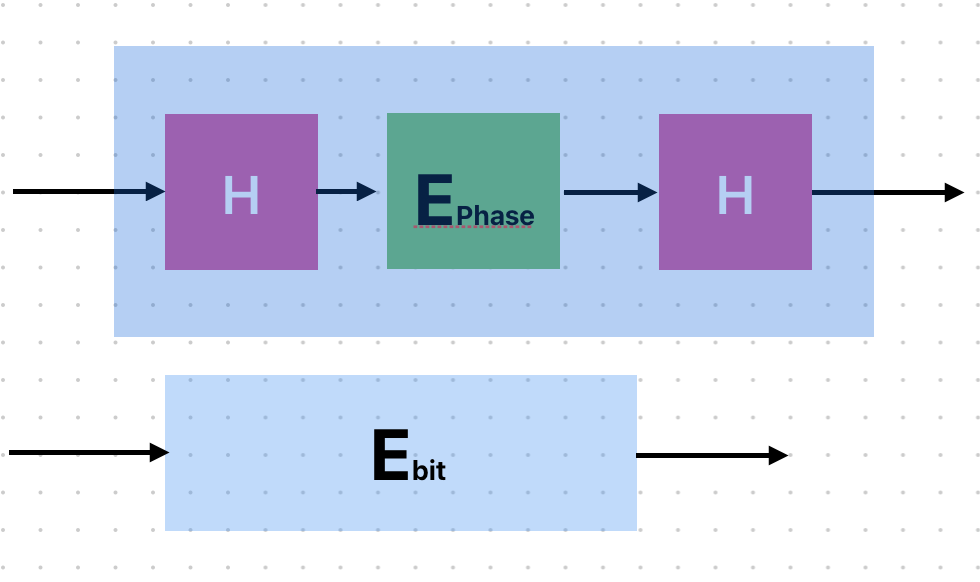
\includegraphics[width=0.7\textwidth]{Figs/BitFlip_equivalence.png}
    \caption{Channel phase-flip noise can be converted to bit-flip noise if we transform the qubit into the basis states \(\ket{+}\), \(\ket{-}\) by applying Hadamard transformation.}
\label{fig:QEC_BitFlipEquivalence}
\end{figure}


\subsection{Combination of bit-flip and phase-flip noise}
It is possible for qubits to experience both bit-flip and phase-flip noise simultaneously. Then the noise model of the channel is 
\[\sigma_X \sigma_Z \; \text{or} \; \sigma_Z \sigma_X\]

Let us against list the transformation by this noise on the two sets of basis states \(\{\ket{0}, \ket{1}\}\), and \(\{\ket{+}, \ket{-}\}\). There are eight cases:  
\begin{align*}
   \sigma_X \sigma_Z \ket{0} &= \ket{1} \\
   \sigma_Z \sigma_X \ket{0} &= -\ket{1} \\
   \sigma_X \sigma_Z \ket{1} &= \ket{0} \\
   \sigma_Z \sigma_X \ket{1} &= -\ket{0} \\
   \sigma_X \sigma_Z \ket{+} &= \ket{-} \\
   \sigma_Z \sigma_X \ket{+} &= -\ket{-} \\
   \sigma_X \sigma_Z \ket{-} &= \ket{+} \\
   \sigma_Z \sigma_X \ket{-} &= -\ket{+}
\end{align*}

\subsection{Other forms of Channel Noise}
Any type of channel noise on a single qubit, including small noises accumulated on the imperfect quantum gates, can be modeled by a unitary matrix multiplication. The unitary matrix of \(2\times 2\), can be decomposed to a linear combination of the four Pauli operators,
\begin{align*}
    E &= \begin{bmatrix}v_{00}&v_{01}\\v_{10}&v_{11}\end{bmatrix} \\
    &= \alpha_0 \begin{bmatrix}1 &0\\0&1\end{bmatrix} + \alpha_1 \begin{bmatrix}0 &1\\1&0\end{bmatrix} + \alpha_2 \begin{bmatrix}1 &0\\0&-1\end{bmatrix} + \alpha_3 \begin{bmatrix}0 &i\\-i&0\end{bmatrix} \\
    &= \alpha_i I + \alpha_1 \sigma_X + \alpha_2 \sigma_Z + \alpha_3 \sigma_Y
\end{align*}

So the (un-normalized) quantum state \(E\ket{\psi}\) can thus be written as a superposition of four terms, \(\ket{\psi}, \sigma_X\ket{\psi}, \sigma_Z\ket{\psi}, \sigma_X\sigma_Z\ket{\psi}\).


Any channel noise thus can be regarded as a tensor product of such linear combination of Pauli operators.  Note that \(\sigma_Y = -i \sigma_X \sigma_Z \). Therefore,  
if we can correct \(\sigma_X,\) and \(\sigma_Z\), we can correct any quantum error!

\subsection{The digitization of Quantum Noise}
Taking the set of qubits and the environment as a whole, then the evolution of the quantum state can be expressed in the form:
\begin{align}
\ket{\phi}\ket{\psi_{0}}_{e} \rightarrow \sum_i (E_i \ket{\phi}\ket{\psi_{i}}_{e} \label{eq:QuantumNoise}    
\end{align}
where each ‘error operator’ \(E_i\) is a tensor product of Pauli operators acting on the qubits, \(\ket{\phi}\) is the initial state of the qubits, and \(\ket{\psi_i}_e\)  are states of the environment. We thus express general noise and/or decoherence in terms of Pauli operators \(\sigma_X, \sigma_Y, \sigma_Z\) acting on the qubits. For clarity, we use denote \(X= \sigma_X, Z=\sigma_Z, Y=-i\sigma_Y = XZ\).

To write tensor products of Pauli matrices acting on \(n\) qubits, we introduce the notation \(X_uZ_v\) where \(u\) and \(v\) are \(n\)-bit binary vectors. The non-zero coordinates of \(u\) and \(v\) indicate where \(X\) and \(Z\) operators appear in the product. For example,

\begin{align}
    X \otimes I \otimes Z \otimes Y \otimes X = X_{10011} Z_{00110}.
\end{align}

Error correction is a process which takes a state such as \(E_i\ket{phi}\) to \(\ket{\phi}\). Correction of \(X\) errors takes \(Z_v\ket{phi}\)  to \(X_uZ_v\ket{phi}\); correction of \(Z\) errors takes \(X_uZ_v\ket{phi}\)  to \(X_u\ket{phi}\). Putting all this together, we discover the highly significant fact that to correct the most general possible noise, it is sufficient to correct just \(X\) and \(Z\) errors.


\section{Repetition Codes}
The first example of a Quantum error correction code is inspired by the repetition code in the classical world. 

\subsection{Review of the Classical Repetition Code}
If we send a single bit over a binary symmetric channel, one simple scheme offering protection is to encode the bit by repeating it multiple times, so that we can use the repetition at the receiver side. This is known as repetition codes. Assume we repeat three times, to transmit a \(0\) we send three bits (sequentially) in the state \(0\), and likewise for \(1\). We can say the encoder encodes the message bit as the following:
\begin{align*}
    0 &\rightarrow 000 \\
    1 &\rightarrow 111      
\end{align*}

Once the three bits have been received, after the noise, where each bit has probability \(p\) being flipped to the opposite bit, they are decoded by a “majority vote”. This intuitive decoding scheme guarantees that any single error is corrected. 

The majority vote decoding assumes measurement of the data bits, which is infeasible in quantum computation - measurement destroys quantum information. A different decoding method is to use syndrome decoding. We check parity by calculating the syndrome \((r_1+r_2, r_1+r_3)\), where \(r_i\) is the \(i\)-th received bit. In accordance of the syndrome, the decoder flips the corresponding bit: 
\begin{align*}
    00 &\rightarrow \text{No flip}   \\
    01 &\rightarrow \text{flip bit \(r_3\)} \\    
    10 &\rightarrow \text{flip bit \(r_2\)} \\  
    11 &\rightarrow \text{flip bit \(r_1\)}     
\end{align*}


For the decoding to fail (the decoder does not return the original transmitted bit), it must be true that either two of the three bits have been flipped (which can occur in three different ways), or all three have been flipped. So the decoding error probability is:
\[p'_{e} = 3 p^2 (1-p) + p^3,\]
which is less than \(p\) if \(p < 0.5\). Typically, \(p\) is small, and we can describe this as the error is reduced to \(O(p^2)\).

We would like to use the repetition idea in the quantum world. Even though the no-cloning theorem dictates that we cannot clone the qubits, we can use entanglement to effectively realize repetition. 

\subsection{The Three qubit code to correct one single bit-flip error}
The three-bit repetition code guarantees to return the correct bit value, so long as at most one of the bits in the code is flipped. We now use this as inspiration for the three-qubit code that can correct one single bit flip error. In the encoding, entanglement plays the role of the repetition. 

Figure~\ref{fig:QEC_BitFlip} shows the 1 logic qubit and 3 physical qubit quantum circuit that is enable to correct upto one single bit flip error. The figure shows three components: the encoder, the noise channel, and the decoder. The encoder entangle two ancillary qubit \(\ket{0}\) to the logic qubit so that for any input basis state \(\ket{b}\), the output is \(\ket{bbb}\),  based on two CNOT gates.

\begin{figure}[ht]
\centering
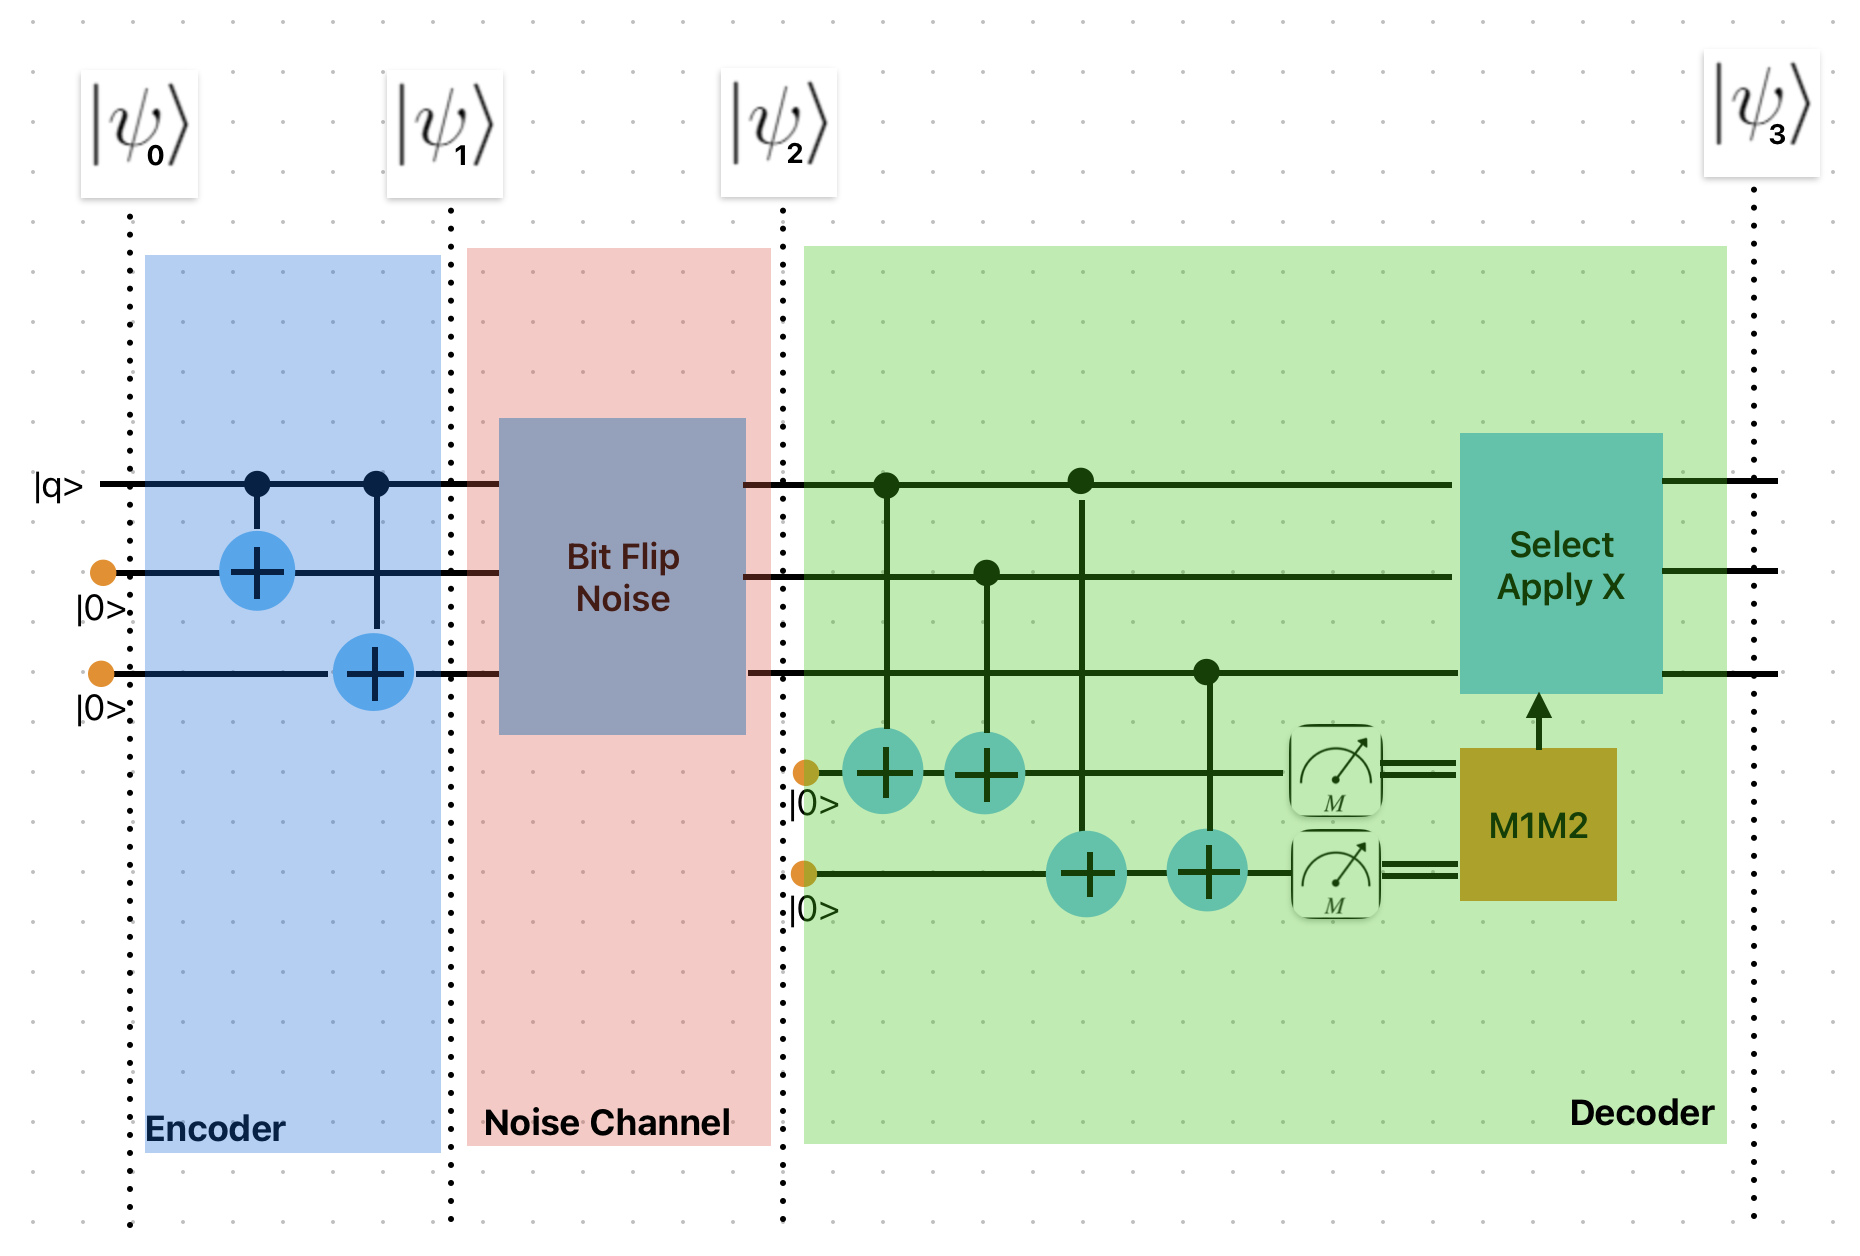
\includegraphics[width=0.98\textwidth]{Figs/QEC_BitFlipCorrect.png}
    \caption{Simple example illustrating the principles of quantum error correction. 
we want to transmit a single-qubit state \(\ket{\q} = \alpha \ket{0} + \beta\ket{1}\). The channel  introduces \(\sigma_X\) errors randomly. Encoder prepares two further qubits in the state \(\ket{0}\), represented by a small yellow circle, 
 and encodes the single qubit into a joint state of three qubits, by two controlled-not operations.
These three qubits go through the noisy channel. At the receiver end, the decoder recovers the joint state by extracting a
syndrome, and applying \(\sigma_X\) operation to one (or none) of the qubits based on the syndrome.}
    \label{fig:QEC_BitFlip}
\end{figure}


That is, we encode the computational basis states:
\begin{align*}
\ket{0} &\rightarrow \ket{\hat{0}} = \ket{000} \\
\ket{1} &\rightarrow \ket{\hat{1}} = \ket{111} 
\end{align*}

where \(\ket{\hat{0}}, \ket{\hat{0}}\) have the meaning of the logical \(\ket{0},\ket{1}\) qubits. Therefore for a general qubit \(a\ket{0} + \beta\ket{1}\), the output state is  
\[\alpha\ket{000} + \beta\ket{111} = \alpha \ket{0}^{\otimes3} + \beta \ket{1}^{\otimes3}.\]

Put together, the quantum encoder encodes the logic qubit \(a\ket{0} + \beta\ket{1}\) into three physical qubits through entanglement. In Figure~\ref{fig:QEC_BitFlip}, let us mark the joint qubits: 
\begin{align*}
\ket{\psi_0} &= (\alpha\ket{0}+\beta\ket{1})\ket{0}^{\otimes2}, \\ 
\ket{\psi_1} &=\alpha\ket{000}+\beta\ket{111}.    
\end{align*}

After passing through the bit-flip channel, the 3-qubit basis states \(\ket{000}, \ket{111}\) might have experienced zero, one, two, or, three qubit flips or errors. Just like classical repetition codes, at this stage, it seems we introduce more errors by doing entanglement. We will show, however, that now we can correct any single bit error and thus reduce the error rate. 

There are four output possibilities with the encoded qubits being distorted assuming at most one bit flip error:

\begin{table}[ht]
\caption{Outcome possibilities for a three qubits repetition code with at most one single error}
\begin{center}
\begin{tabular}{ |c |c | c | }
\hline
input & \text{Error Event} & Output (\(\ket{\psi_2}\))\\
\hline
\(\alpha\ket{000}+\beta\ket{111}\) & \text{no bit flipped} & \(\alpha \ket{000} + \beta \ket{111}\) \\
&\text{first qubit flipped} & \(\alpha \ket{100} + \beta \ket{011}\) \\
&\text{second qubit flipped}  & \(\alpha \ket{010} + \beta\ket{101}\) \\
&\text{third qubit flipped}  & \(\alpha \ket{001} + \beta \ket{110}\) \\
\hline
\end{tabular}
\end{center}
\end{table}


At the receiver end, receiving the corrupted \(3\)-qubit, the decoder now introduce two more qubits, prepared in the state \(\ket{00}
\). This extra pair of qubits, referred to as an ancilla, is not strictly necessary, but makes error correction easier to understand. The ancilla qubits are used to gather information about the noise. As discussed in the previous chapter, controlled-NOTs from the first and second received qubits to the first ancilla qubit computes the parity checks on the first two received qubits; controlled-NOTs from the first and third received qubits to the second ancilla bit computes the parity checks on the first and third received qubits. Measuring the two ancilla bits to the basis \(\{\ket{0} , \ket{1}\}\) gives two classical bits of information, we have a syndrome \(M_1, M_2\), completely analogous to the classical repetition codes. The error syndrome locates the error in the received qubits. Based on the syndrome, the decoder apply a Pauli swap matrix \(\sigma_X\) to one of the qubit to correct it. Suppose for example the decoder's syndrome is \(10\) (i.e. the ancilla state is projected onto \(\ket{10}\)). We see that the state of the received qubits must be  \(\alpha\ket{010} + \beta \ket{101}\) if there is at most one error, which means the second bit experienced bit flip. We can orrect the state by applying a Pauli \(\sigma_X\) operator to the second qubit. He thus obtains \(\alpha\ket{000} + \beta\ket{111}\).


\begin{table}
\caption{Syndrome \(M_1\M_2\) in Figure~\ref{fig:QEC_BitFlip}; and based on the syndrome, the decoder applies \(\sigma_X\) to the corresponding qubit. Finally, we see the \(\psi_3\) is always the original input, given the bit flip error is at most at one qubit.}
\begin{center}
\begin{tabular}{ |c | c | c | c |c |}
\hline
Bit-flip & \(\ket{\psi_2}\) & \(M_1 M_2\) & Recovery & \(\ket{\psi_3}\) \\
\hline
-  & \(\alpha \ket{000} + \beta\ket{111}\) & 0 0 & \(I \otimes I \otimes I\) & \(\alpha \ket{000} + \beta\ket{111}\) \\ 
1 & \(\alpha \ket{100} + \beta\ket{011}\) & 1 1 & \(\sigma_X \otimes I \otimes I\) & \(\alpha \ket{000} + \beta\ket{111}\)\\
2 & \(\alpha \ket{010} + \beta\ket{101}\) & 1 0 & \(I \otimes \sigma_X \otimes I\) & \(\alpha \ket{000} + \beta\ket{111}\)\\
3 & \(\alpha \ket{001} + \beta\ket{110}\) & 0 1 & \(I  \otimes I \otimes \sigma_X\) & \(\alpha \ket{000} + \beta\ket{111}\)\\
\hline

\end{tabular}
\end{center}
\end{table}


That is, we have made comparative parity-check measurements that tell us only about the error and not about the quantum state itself, and so these measurements have not destroyed the quantum state.

\paragraph{class break}

\subsection{A Simplied three qubit code for bit-flip error}
As we mentioned, the ancilla qubits introduced at the decoder is not strictly necessary. If we are only interested in having \(\ket{\psi}\) robust against at most one qubit bit-flip, then Figure~\ref{fig:QEC_BitFlipSimplied} shows a simplied quantum logic. 

\begin{figure}[ht]
\centering
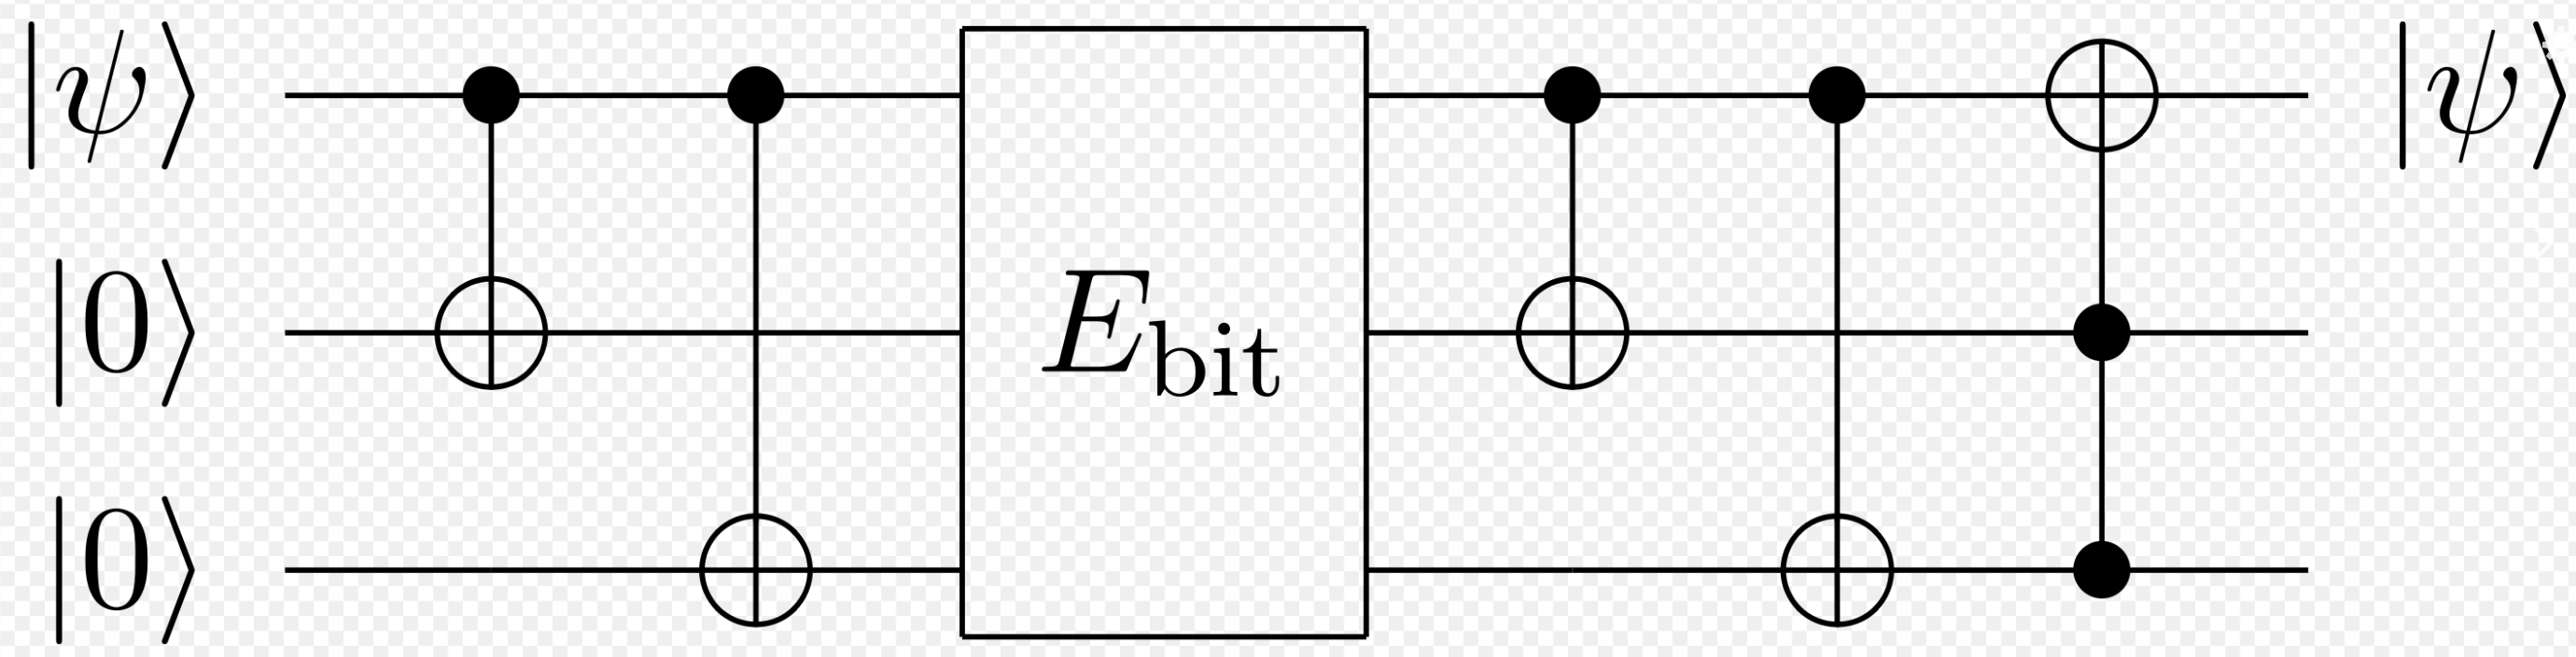
\includegraphics[width=0.98\textwidth]{Figs/QEC_BitFlipSimplified.png}
    \caption{Simplified three qubit encoder/decoder which is robust against one bit-flip noise. A control-control-not circuit swaps the first qubit if the syndrome indicates that this qubit is swapped by the channel noise \(E_{bit}\)}
\label{fig:QEC_BitFlipSimplied}
\end{figure}


\subsection{The Three qubit Phase Flip Code}
As discussed in Section 3.2, a phase flip noise can be treated as a bit flip noise if we transform an original state of the qubit in bases \(\{\ket{0}, \ket{1}\}\) to bases \(\{\ket{+}, \ket{-}\}\) by applying Hadamard operation before the channel, but applying Hadamard operation again after the channel. With this trick, the three qubit bit flip code can be used to correct a single phase flip error as well. 

This is depicted in Figure~\ref{fig:QEC_PhaseFlipSimplied}.  

The original state of the qubit 
\[\ket{\psi} = \alpha \ket{0} + \beta\ket{1}.\]

First, through the entanglement, we have 
\[\alpha \ket{000} + \beta\ket{111}.\]

Second, after the Hadamard transformation, we have
\[\alpha \ket{+++} + \beta\ket{---}.\]

The block \(E_{phase}\) introduces at most one phase-flip noise, so the output state is one of the following four states:
\begin{align*}
& \alpha \ket{+++} + \beta\ket{---}.\\
& \alpha \ket{-++} + \beta\ket{+--}.\\
& \alpha \ket{+-+} + \beta\ket{-+-}.\\
& \alpha \ket{++-} + \beta\ket{--+}.
\end{align*}

After the Hadamard transformation, we have the possible states are:
\begin{align*}
& \alpha \ket{000} + \beta\ket{111}.\\
& \alpha \ket{100} + \beta\ket{011}.\\
& \alpha \ket{010} + \beta\ket{101}.\\
& \alpha \ket{001} + \beta\ket{110}.
\end{align*}
Therefore, a syndrome decoding will correct the possible phase-flip error and return the original qubit \(\ket{\psi}\).



\begin{figure}[ht]
\centering
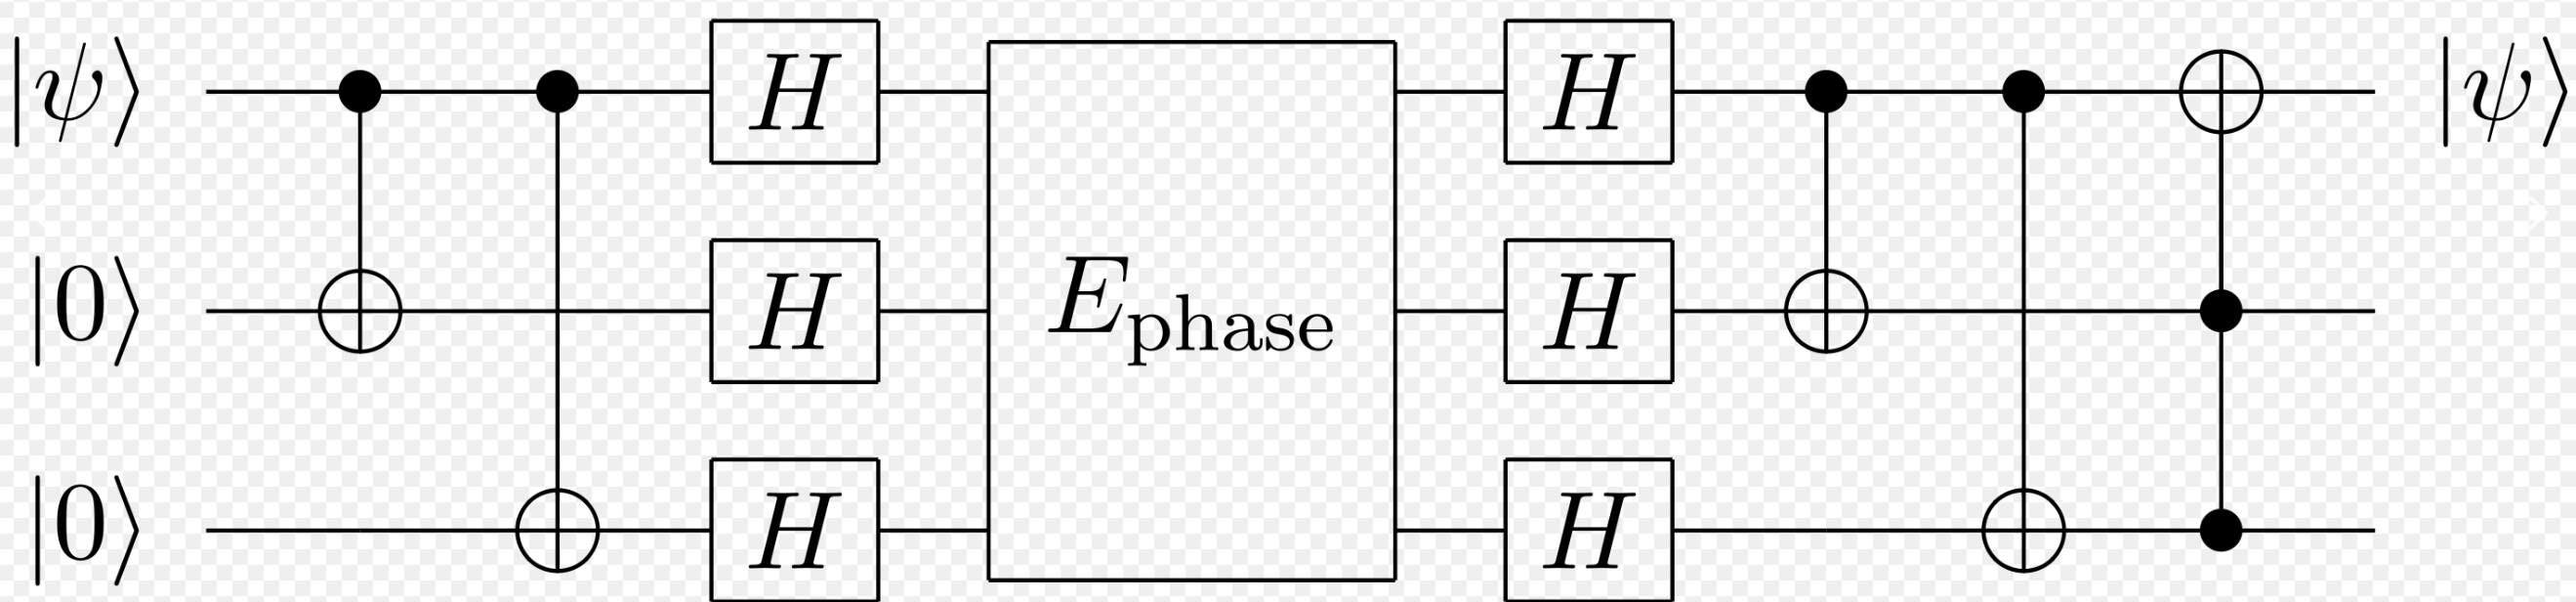
\includegraphics[width=0.9\textwidth]{Figs/QEC_PhaseFlipSimplified.png}
    \caption{Simplified three qubit encoder/decoder which is robust against one phase-flip noise. }
\label{fig:QEC_PhaseFlipSimplied}
\end{figure}



\section{Shor's Code}
Now we consider case that the error channel may induce either a bit flip, a phase flip, or both. It is possible to correct for both types of errors on any one qubit using a QEC code, which can be done using the Shor code published in 1995. This is equivalent to saying the Shor code corrects arbitrary single-qubit errors. The basic idea is to concatenate the two codes we introduced earlier: the 3 qubit code to correct a bit flip and the 3 qubit code to correct a phase flip. 

\subsection{The \(3\) qubit bit-flip code in the presence of phase-flip error}
What if we use the \(3\) qubit bit-flip code on an error channel that may have both bit-flip and phase-flip single error? 

We know that the \(3\) qubit bit-flip code guarantees to correct any single bit-flip error. If there is a phase flip error, in addition to a bit flip error, the return state could be either \(\alpha\ket{0} + \beta \ket{1}\) or \(\alpha\ket{0} - \beta \ket{1}\). That is, with the \(3\) qubit bit-flip code, such a channel becomes a channel only with phase flip error.


\subsection{Shor's code}
The code is structured as a tensor product of three structurally identical blocks. In each of the block, a qubit is first transformed by the Hadamard matrix and then entangle two ancillary \(\ket{0}\) by CNOT gate to produce 
\begin{align*}
    \ket{0} &\rightarrow \ket{000} + \ket{111}  \\
    \ket{1} &\rightarrow \ket{000} - \ket{111}  \\
    \alpha\ket{0} + \beta \ket{1} &\rightarrow \alpha(\ket{000} + \ket{111}) + \beta(\ket{000} + \ket{111})  
\end{align*}

So the total \(9\) physical qubit code for the logic qubit \(\ket{\psi} = \alpha\ket{0} + \beta \ket{1}\) is:

\begin{align}
   \alpha\ket{0} + \beta \ket{1} &\rightarrow \alpha \ket{0_S} + \beta \ket{1_S} \label{eq:ShorCode}
\end{align}
where, 
\begin{align*}
    \ket{0_S} &= \frac{1}{2\sqrt{2}}(\ket{000} + \ket{111})^{\otimes 3},\\
    \ket{1_S} &= \frac{1}{2\sqrt{2}}(\ket{000} - \ket{111})^{\otimes 3}.\\
\end{align*}

Although the circuit looks daunting, the analysis of it is simple and can be thought of a two step decoding process. 

The first step is to decode the inner \(3\) qubit code that corrects one single bit flip error in each of the \(3\) blocks. As discussed in Section 5.1, from the perspective of the logic qubits after the Hadamard matrix, the channel is equivalent to a channel with phase flip error only. 
So the whole channel now becomes a phase flip error channel and the 3 qubit code, taken as from line 1, 4, 7, can correct. 







\begin{figure}[ht]
\centering
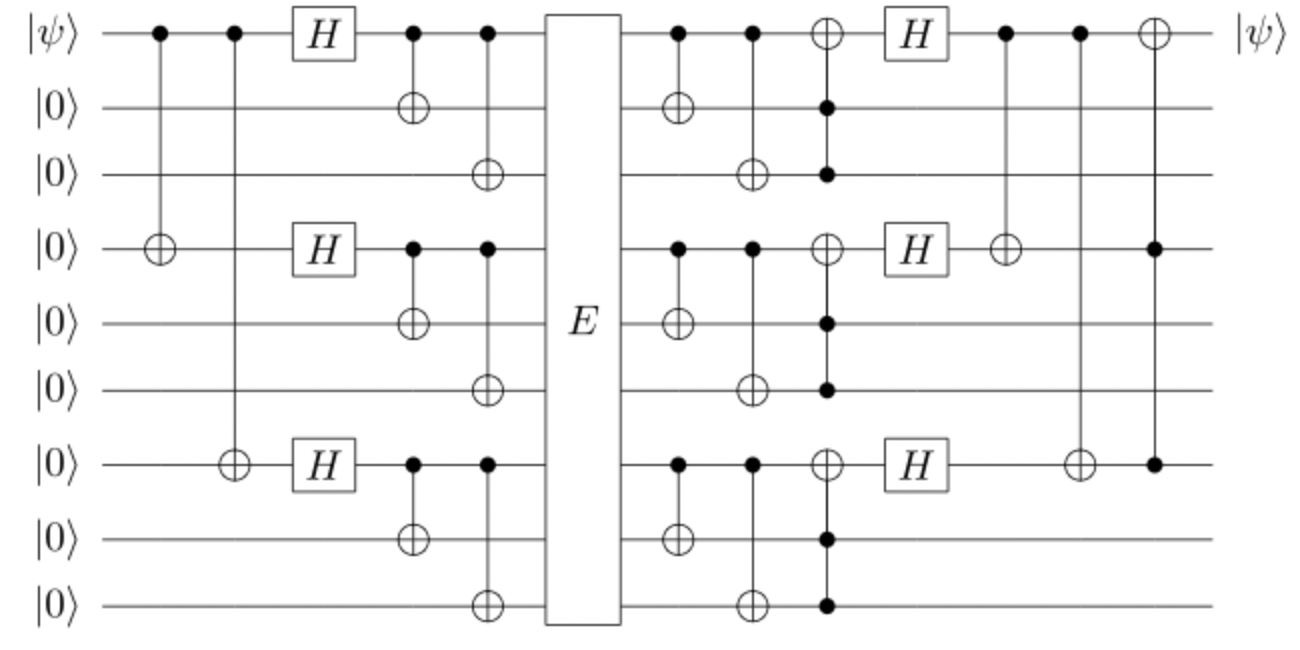
\includegraphics[width=0.9\textwidth]{Figs/QEC_ShorsCode.png}
    \caption{Shor's 9 qubit code that is robust against any single bit flip and phase flip error.}
\label{fig:QEC_Shor}
\end{figure}


\section{Exercise}
\begin{enumerate}
    \item Show the encoding part of the circuit in Fig. 4 does what it is supposed to, i.e., an initial \(\ket{+}\) is encoded as \(\ket{+++}\), and \(\ket{-}\) as \(\ket{---}\).
    
    \item Construct the code that allows correction of a \(Y\) error if it occurs on only one carrier, and design the corresponding coding and decoding circuit. [Hint: One should replace \(H\) in Fig. 4 with something else. What should it be?]
    
    \item Show that the encoding circuit in Fig. 5 produces the result in Eq.~\ref{eq:ShorCode}.

\end{enumerate}